\pdfoutput=1

\documentclass{4thYearProject}

\makeatletter\@openrightfalse\makeatother
\usepackage{graphicx}
\usepackage{tabularx}
\usepackage{diagbox}
\usepackage{hyperref}
\usepackage{float}
\usepackage{longtable}
\usepackage{listings}
\usepackage{color}
\usepackage{pdfpages}

% Used for subsubsections%
\usepackage{titlesec}
\setcounter{secnumdepth}{4}
\setcounter{tocdepth}{4}

\definecolor{dkgreen}{rgb}{0,0.6,0}
\definecolor{gray}{rgb}{0.5,0.5,0.5}
\definecolor{mauve}{rgb}{0.58,0,0.82}

\newcolumntype{Y}{>{\raggedleft\arraybackslash}X}

\graphicspath{ {resources/images/} }

\begin{document}
\title{Microissues IntelliJ Plugin}
\author{Alex Leet}
\date{2016/2017}
\maketitle

\begin{abstract}
Abstract here
\end{abstract}

\educationalconsent

\tableofcontents
%==============================================================================

\chapter{Introduction}
\pagenumbering{arabic}

\section{Project Context}



\section{Motivation}

The majority of issue management systems are either client-server applications, distributed or hosted systems. Based on the research described in section \ref{sec:Research} and the already existing plugins, there is a lack of attempts of reducing context switch between using issue management systems and computer programming. 

\section{Objectives}

The prime objective of the project is to develop a working plugin with minimal features that demonstrate the concept of how a source code integrated issue management system could work, which will then be used for user evaluation including gathering feedback to gain an understanding of users' perspective on how it compares to traditional issue tracking.

\section{Achievements}

The plugin developed conforms to the initial idea and the requirements and has undergone user evaluation in order to confirm the working of it. Survey on usability and informal opinion on how the users felt the plugin compared to the issue tracking systems they have previously used was conducted, of which the results will be described in \ref{sec:usereval}.

\section{Dissertation Structure}

The dissertation will follow the structure outline in the below table \ref{table:reportStructure}.

\begin{table}[H]
\centering
\def\arraystretch{1.5}
\begin{tabular}{p{3cm}p{12cm}}
\hline
Chapter & Content \\
\hline
2. Background & A short description of the previous work related to the project and research done on issue management. \\
3. Requirements & Discusses the gathering of the requirements, followed by a list of all requirements. \\
4. Design & Details the design decisions taken and contains a list of final design features.\\
5. Architecture & Describes the implementation aspects of the plugin throughout development\\
6. Evaluation & Describes the test process and the user evaluation carried out, their results and a discussion of the results. \\
7. Conclusion: & Discusses the outcome of the project, future work possibilities and learning outcomes.  \\
\hline
\end{tabular}
\caption{Dissertation Structure}
\label{table:reportStructure}
\end{table}


\chapter{Background}

This chapter discusses the specifics of issue tracking systems and outlines related work - in particular the already existing plugins relating to issue tracking and also discusses research on how developers perceive issue tracking and what part it plays in their software development process.

\section{Issue Tracking}

Issue tracking is the process of documenting and keeping track of tasks or defects that occur during development. It is considered to be a vital part of software development process and can be considered as a means of communication within the development team \cite{socialnature}.

\subsection{Issue Tracking Systems}

An issue tracking system is a computer software that is used create and track the aforementioned issues. They essentially act as databases that store all the relevant information pertaining the status updates on issues from their creation to completion \cite{socialnature}. % Possibly add more here saying different issue management systems have different customisability and features?

% Should this be called "Tickets" or "Issues"?
\subsection{Tickets}

In issue tracking systems the electronic artefacts representing a particular task, bug, epic or story are commonly known as issues or tickets. They contain various information with the most common fields being:

\begin{itemize}
\item \textbf{Summary} - The summarization of the purpose of the ticket.
\item \textbf{Type} - The type of the ticket, most commonly either a task, bug, user story or an epic. 
\item \textbf{Status} - At which stage the completion of the ticket is in.
\item \textbf{Priority} - The importance of the ticket compared to other tickets.
\item \textbf{Resolution} - Why the ticket was set as completed.
\item \textbf{Assignee} - Who is responsible for completion of the ticket.
\item \textbf{Estimated time} - How long the completion of the ticket is estimated to take.
\end{itemize}

In addition to the above mentioned, the available fields of entry can vary from one system to another and in some, custom creation of fields according to a team's needs is possible. 

\section{Related Work}

Various plugins have been developed to ease the integration of issue management and integrated development environments (IDEs). However, as the below mentioned examples will demonstrate, most are intended to connect to the various issue management systems available. 

\subsection{Inbuilt IntelliJ Task Management Plugin}

%Might have the ability to create local tasks%
IntelliJ IDEA is bundled with its own task management plugin and is activated by default. It allows for integration to various issue tracking systems, which gives the user the functionality to open, create and delete tasks or issues. Therefore a server that the tasks and issues are hosted on is necessary to use the inbuilt feature, which means there is no capability to create tickets locally. Additionally, tickets cannot be linked to source code in any way.

\begin{figure}[H]
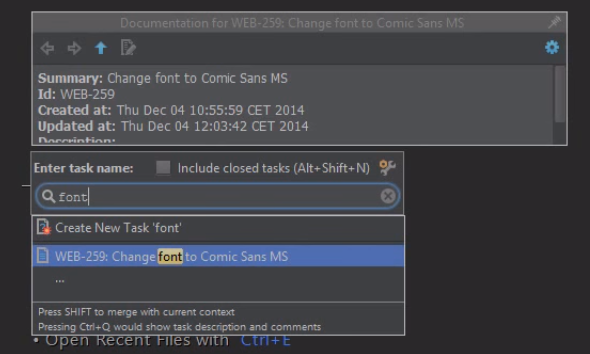
\includegraphics[scale=0.5]{IntelliJ_Tasks}
\centering
\caption{Example of viewing a YouTrack task in IntelliJ}\label{intellijtask}
\label{fig:intellijtask}
\end{figure}

\subsection{Tasks Navigation Plugin}

An attempt to connect source code to issue management systems in order to reduce context switch was attempted by Vladislav Rassokhin, who developed the plugin \textit{Tasks Navigation} that allows the user to link to issues in the Web from comments and reference injections in IntelliJ \cite{tasksnavigation}. With the plugin it is easy to quickly get information about the issue and to see which part of code the issue particularly pertains to. 

\begin{figure}[H]
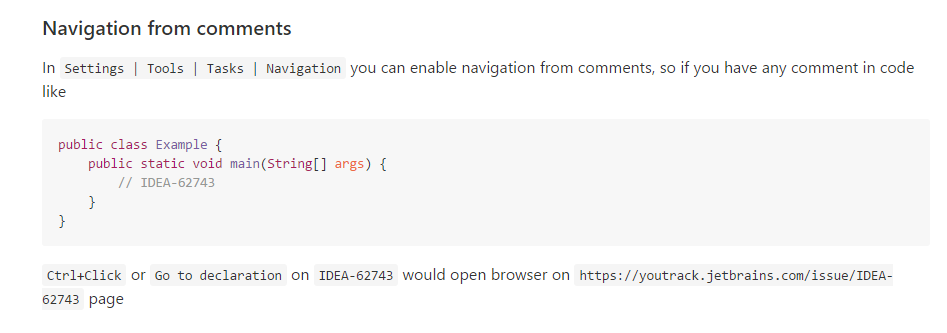
\includegraphics[scale=0.6]{Tasks_Navigation_Plugin}
\centering
\caption{Example of how the Tasks Navigation plugin works}\label{tasksnavigation}
\label{fig:tasksnavigation}
\end{figure}

\subsection{Tasks Plugin}

Another IntelliJ plugin that was developed by Sergiy Dubovik and continued by Warner Jan Veldhuis is Tasks, which allows the user to locally manage tasks and issues. The plugin has a well structured interface featuring a wide array of capabilities such as creating, removing and editing tasks. The plugin also includes the ability to assign priorities to tasks and keep track for how long they have been worked on. However, there is no possibility to connect the tasks to source code. 

\begin{figure}[H]
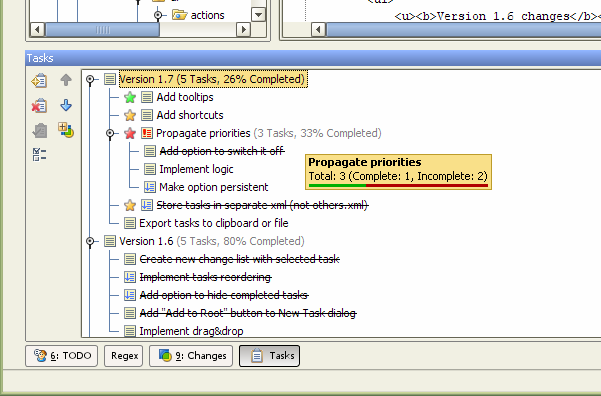
\includegraphics[scale=0.6]{Tasks}
\centering
\caption{Example of task management in the Tasks plugin}\label{tasks}
\label{fig:tasks}
\end{figure}

\subsection{Mylyn}

Mylyn is the task and application lifecycle management (ALM) framework for Eclipse. It boasts a wide array of features, including being able to work on either local tasks, which do not require a shared repository, or shared repository tasks, which do. 

\subsection{Eclipse TODO Editor Plugin}

The Eclipse todo editor plugin that allows to edit todo files in Eclipse. 

\begin{figure}[H]
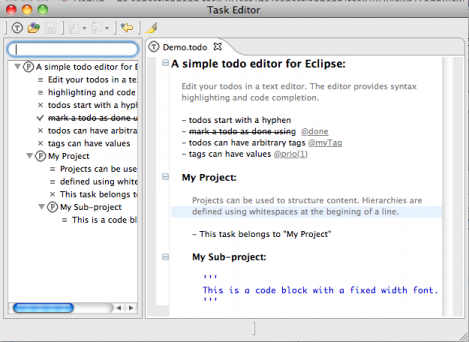
\includegraphics[scale=0.6]{eclipse_TODO_editor}
\centering
\caption{Example of the editor window, including the visual display of todo's on the left}\label{eclipsetodo}
\label{fig:eclipsetodo}
\end{figure}

\subsection{Summary of Related Work}

All of the above mentioned plugins were developed with a specific purpose in mind. However, they can be mainly divided into two categories:

\begin{itemize}
\item Plugins intended to be used with an already existing issue management system available. 
\item Plugins that act as standalone issue management systems themselves.
\end{itemize}



\begin{center}
\begin{table}[H]
\noindent
\begin{tabular}{|l|*{5}{c|}}\hline
\backslashbox[50mm]{Plugin}{Feature}
&\makebox{Integration with source code}&\makebox{Local issue management}&\makebox{Display of all issues}
\\\hline
IntelliJ Inbuilt Plugin & Yes &&\\\hline
Tasks Navigation & No &&\\\hline
Tasks & Yes & &\\\hline
Mylyn & No & & \\\hline
Eclipse TODO Editor & Yes && \\\hline
\end{tabular}
\label{table:featurematrix}
\caption{Feature matrix of related plugins}
\end{table}
\end{center}

\section{Research on Issue Tracking and Usage of Issue-tracking Systems}\label{sec:Research}

Attempts have been made to research recording of issues and bugs and the common shortcomings of how bugs and issues are documented. A study by Jorge Aranda and Gina Venolia has found that one of the most crucial bits of information missing in issue management is links to source code and the change-sets that resolved these bugs \cite{lifeofbugs}. Additionally, they had found that in some cases, the key events in the story of a bug had left no electronic trace and therefore there was no way to discover the important information pertaining the fixing of a bug.

One of the interview results in the research paper "How Software Engineers Use Documentation: The State of the Practices" is that software engineers value documentation that requires little effort but still serve as important historical information and such code-level comments are one of the most preferred methods of documentation since they are short and rest within the source code, therefore resulting in very little maintenance work  \cite{stateofpractice}. 

\section{Evaluation of Related Work and Related Research}

Taking into consideration the main points which were considered when reviewing the already existing plugins (integration with source code, local issue management and display of all isues), it is clear that none of the plugins are completely standalone issue management systems which are integrated with source code. 
From the research it is evident that using an issue management system is an important part of development process, however, the fact that it is usually widely separate from the source code is a decremental aspect. 

\chapter{Requirements}



\section{Requirements Elicitation and Gathering}

Project requirements were gathered and discussed throughout weekly meetings with Dr. Timothy Storer of Computing Science department at the University of Glasgow. Both functional and non-functional requirements had to be carefully considered due to the fact that the aim of the plugin was a working plugin with enough minimal features that would allow to gather feedback an source-code integrated issue management and how it compares to standard issue management. 

%https://ocw.mit.edu/courses/aeronautics-and-astronautics/16-885j-aircraft-systems-engineering-fall-2005/readings/sefguide_01_01.pdf%

\section{Functional Requirements}

Functional requirements define what the system must be able to do and are defined as features of the system. 

\subsection{Allow the User to Create Tickets}

In order for the plugin to function as a local issue management system, the ability for the user to create tickets is a key feature to be included. Due to the nature of the project, the tickets have to explicitly reside in the source code and therefore a way for the user to explicitly signify a ticket has to be considered.

\subsection{Detect User Created Tickets}

The created tickets should be detected by the plugin, either as they are being created or after the user has finished creating the ticket.

\subsection{Display the Tickets}

The detected tickets should be displayed in order for the user to get an overview of all the issues created.

\subsection{Display Ticket Information}

Ticket information has to be displayed when a particular ticket is selected and must include all the relevant information that the user has specified when creating the ticket.

\subsection{View a Ticket's History}

Ticket's history throughout version control commits has to be retrieved with the appropriate changes indicated, including the information relating to the commit itself - the date and the committer details.

\section{Non-Functional Requirements}

Non-functional requirements describe what qualities the system should have and their primary objective is to ensure the satisfaction with the system \cite{nonfunctional}.

\subsection{Usability}

The creation and management of tickets should be simple, quick and not require expert knowledge. The user should be able to get help on how to use the plugin relatively quickly.

\subsection{Performance}

The plugin should not impact the overall performance of the IDE. The ticket creation, detection and display should therefore be relatively fast in order to match the performance of other features of the IDE in order not to disrupt the workflow of the developer. 

\subsection{Reliability}

The plugin should not be prone to crashes and exceptions. In the case crashes do occur, they should not prevent the user from using any other features of the IDE apart from the ones relating to the plugin.  

%http://www.bredemeyer.com/pdf_files/NonFunctReq.PDF%

\chapter{Design}

The design of the plugin followed iterative development cycles and follows a similar style of the other features in the IDE. 

\section{Main Tool Window}

The plugin features an openable tool window anchored to the bottom of the IDE and is the main mean of displaying information to the user. The tool window is separated into the following components: 

\begin{itemize}
\item Toolbar for helper commands
\item Ticket tree display
\item Ticket information display
\end{itemize}

\subsection{Toolbar}\label{sec:toolbar}

The toolbar is responsible for providing helper commands, which are visualised as clickable icons, to the user. \newline
From top to bottom the commands are:
\begin{itemize}
\item Display help dialog
\item Refresh all the tickets
\end{itemize}

\begin{figure}[H]

\includegraphics[scale=0.6]{Toolbar_figure}
\centering
\caption{The toolbar with the helper command icons: refresh (top), help dialog (bottom)}\label{toolbar}
\label{fig:toolbar}
\end{figure}

% Figure here %
\subsubsection{Help dialog}

The help dialog presents the user the information on what the plugin does and how ticket creation works. 

\begin{figure}[H]
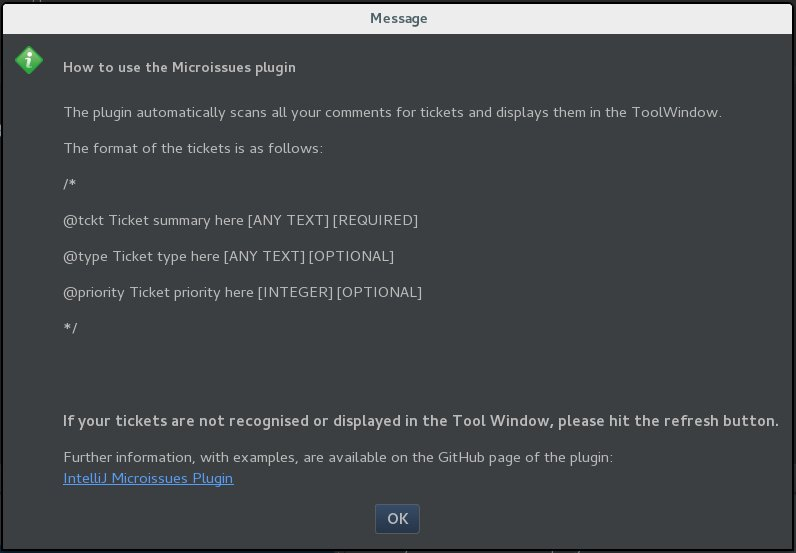
\includegraphics[scale=0.6]{HelpDialog}
\centering
\caption{The displayed help dialog after the user clicks on the icon}\label{helpdialog}
\label{fig:helpdialog}
\end{figure}

% Figure here %

\subsubsection{Refresh command}

The refresh command refreshes all the tickets in the case that there are discrepancies between the tickets they have typed and the tickets that are displayed in the ticket tree.

\subsection{Ticket Tree Panel}

The ticket tree panel contains a scrollable pane that contains a tree of all the tickets. Each of the nodes correspond to either:
\begin{itemize}
\item Ticket Summary, if the ticket is a ticket in the source code. 
\item Change details and commit date if the ticket is an older version of the ticket. 
\end{itemize}

% Figure here %

%FIX THIS%
From this example, we can see that the ticket with the summary "<SUMMARY HERE>" has an older version, with the change indicated as "<CHANGE HERE>". 

\subsection{Ticket Information Panel}

The ticket information panel displays information about the ticket. Similarly to the ticket tree, there is a distinction between the information displayed for a current ticket and an older ticket. The distinction is as such:

\begin{itemize}
\item Current ticket - Ticket information is displayed for all the available information of the ticket.

\begin{figure}[H]
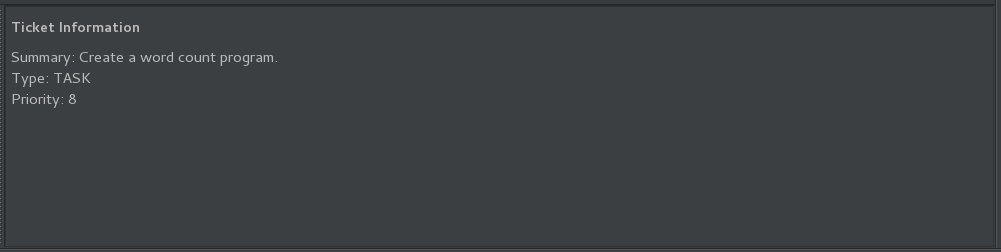
\includegraphics[scale=0.6]{Ticket_infopanel}
\centering
\caption{The panel displaying ticket information.}\label{ticketpanel}
\label{fig:ticketpanel}
\end{figure}

\item Old ticket - In addition to the above details, the old ticket additionally has the commit information (the date and the committer) and which fields are different.
\end{itemize}

\begin{figure}[H]
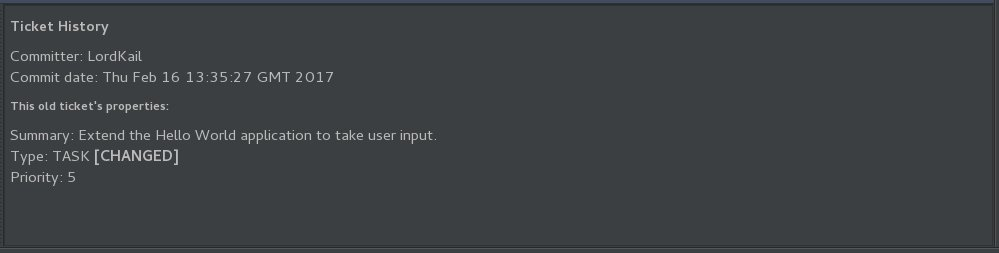
\includegraphics[scale=0.6]{OldTicket_infopanel}
\centering
\caption{The panel displaying an older ticket's information.}\label{oldticketpanel}
\label{fig:oldticketpanel}
\end{figure}

% Two figures here %

\chapter{Architecture}

The development process for most of the components of the plugin has been iterative, with some features requiring a re-design due to the shortcomings in prior implementation techniques that were discovered throughout development. 

The architecture of the plugin will be outlined and discussed in the following sections in the natural order that the plugin operates in. 

\section{Plugin startup}

The initial concern was considering how and when the plugin should be started. Two different approaches were tried:
\begin{itemize}
\item Implementing the \textit{ProjectComponent} interface  
\item Implementin the \textit{StartupActivity} interface 
\end{itemize}

\subsection{ProjectComponent}

The project component is a plugin component, which is associated to a plugin. The implementation class, in this project's case \textit{ToolWindowComponent.java}, becomes a component, which can be accessed from anywhere in the code using the \textit{getComponent(class)} method on an instance of a Project. In order for the implementation to be recognised as a component, it has to be registered in the \textit{plugin.xml} as such:\\

\begin{lstlisting}[language=XML, 
basicstyle={\scriptsize\ttfamily}, 
frame=single,
showstringspaces=false,
breaklines=true,
,tabsize=3]
<project-components>
    <component>
      <implementation-class>uk.ac.glasgow.microissues.ui.ToolWindowComponent</implementation-class>
    </component>
</project-components>
\end{lstlisting}

Initially this approach was used to create the tool window and at the same time, start the process of scanning the files for comments. This approach worked until it was discovered that it threw an exception when the project took a slightly longer time to load. The exception thrown was that PSI elements could not be accessed while the project was loading and therefore a different approach had to be found. 

\subsection{StartupActivity}

The \textit{StartupActivity} interface allows the implementation class to be run after the project has initialized and loaded. This is done by registering it in the \textit{plugin.xml} as a \textit{postStartupActivity}:   \\

\begin{lstlisting}[language=XML, 
basicstyle={\scriptsize\ttfamily}, 
frame=single,
showstringspaces=false,
breaklines=true,
,tabsize=3]
<postStartupActivity implementation="uk.ac.glasgow.microissues.ui.SetupToolWindow"></postStartupActivity>
\end{lstlisting}

It was discovered, however, that this approach did not work for initialising the tool window as during some occurrences it would not appear. However, when it did, it was apparent that an exception when scanning the files for comments was not thrown and that led to the solution.

\subsection{Solution}

The importance of having discussed both of the approaches above is that the appropriate solution found was using a mixture of both of these techniques. 

The \textit{initComponent} and \textit{projectOpened} methods from the \textit{ProjectComponent} interface were used to initialize and register the tool window to the project as a component and using the \textit{runActivity} method from the \textit{StartupActivity} interface allowed to start the process of scanning the files for comments without an exception being thrown.

\section{Tickets}

As tickets reside as comments in the code, a way to extract them and turn them into actual ticket instances was necessary. This was accomplished by utilising Program Structure Interface (PSI) elements, the collection of which represents an internal structure of the source code in the IntelliJ Platform. \\

To store data relating to a particular ticket, the \textit{Ticket} class was created.

\begin{figure}[H]
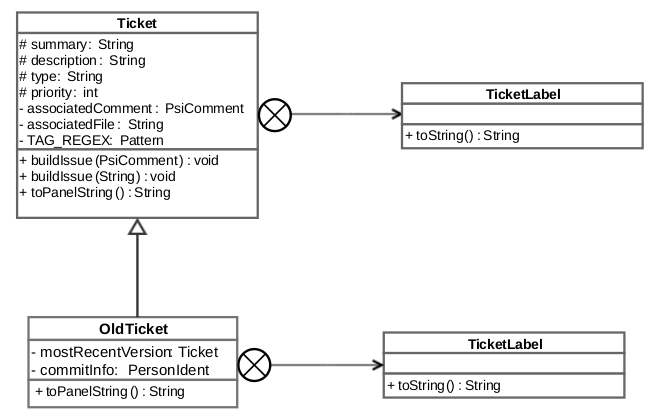
\includegraphics[scale=0.6]{Ticket_UML}
\centering
\caption{The UML diagram of the Ticket class presenting its inner class and the subclass.}\label{ticketuml}
\label{fig:ticketuml}
\end{figure}

\subsection{PSI Tree Traversal \& PSI Comments}

Comments are scanned and found by traversing the PSI tree of the whole project at the start of the plugin. IntelliJ treats comments as instances of \textit{PsiComment} which is a subclass of \textit{PsiElement}.   

\subsection{Ticket Building}

The ticket building is done by extracting the text from the corresponding PSI Element and performing a regular expression matching on the \textit{String}.

The exact regular expression pattern used in the code is:
\begin{lstlisting}[language=Java, basicstyle=\footnotesize\tt,        % the size of the fonts that are used for the code
  frame=single,                    % adds a frame around the code
  language=Java,                 % the language of the code
  keywordstyle=\bf]
 private static final Pattern TAG_REGEX = Pattern.compile("@(.+?)\\s(.+?)\\n");
\end{lstlisting}

For example, this will match lines such as \textit{@tckt Sample summary} and capture the tag "tckt" and the following text "Sample summary". 

\section{PsiTreeChangeListener}

With source-code based tickets, it is important to detect when a comment containing the ticket is added, removed, changed or moved, in order to represent the most current state of the tickets at all times. This removes the necessity for the user to explicitly signify when they have made a change.

The IntelliJ Platform Plugin Software Development Kit (SDK) does not provide a direct way to monitor a particular PSI element. Instead, it provides a \textit{PsiTreeChangeListener} interface that upon implementation listens for changes in the project's PSI tree and invokes the appropriate methods. The particular methods that were used are:

\begin{itemize}
\item public void childAdded(@NotNull PsiTreeChangeEvent event) - invoked when a PsiElement has been added.
\item public void childRemoved(@NotNull PsiTreeChangeEvent event) - invoked when a PsiElement has been removed.
\item public void childReplaced(@NotNull PsiTreeChangeEvent event) - invoked when a PsiElement has been changed.
\item public void childrenChanged(@NotNull PsiTreeChangeEvent event) - invoked when a lot of PsiElements have been changed at once.
\item public void propertyChanged(@NotNull PsiTreeChangeEvent event) - invoked when a PsiElement's property has changed.

\end{itemize}

\subsection{Initial approach}

The initial approach to using the \textit{PsiTreeChangeListener} was to create, delete and update tickets on individual basis based on the corresponding PSI element that was changed. \\
For example, if an already existing comment (which was a ticket) was edited, the associated ticket would be rebuilt based on the newer version of the comment. 

It was discovered, however, that this approach is unstable due to the nature of the PSI elements changing in a very unpredictable manner and in many cases, complex nested statements had to be written in order to ensure that no exception would be thrown due to a lost reference to a PSI element. In addition to exceptions thrown, when a reference to a PSI element was lost it was very . Therefore an alternative approach had to be found.

\subsection{Simplification}

Due to the shortcomings of the previous method, the code was restructured in order to handle changes to the PSI tree differently. \\
The new and currently used simplified method involved associating tickets to the file they reside in. When a PSI element change is detected the following workflow occurs:

\begin{itemize}
\item The PSI element is checked to be a comment and a ticket, if it is:
\begin{itemize}
\item Previous tickets in the task tree relating to the file that the PSI element is in are removed.
\item The file is rescanned for complete tickets and are displayed in the task tree. 
\end{itemize}
\end{itemize}

This ensures that at all times, every single ticket of the file is ensured to be in the task tree without lost references.

\section{Ticket History and Git}

There were various options for selecting an appropriate method for recording ticket history and retrieving ticket history. These included:

\begin{itemize}
\item Associating a ticket with an ID - when the user creates a ticket by writing the comment, an ID would either be generated automatically or they would add an ID themselves and the old ticket versions would be retrieved from version control history by finding tickets with the same ID.
\item Using an approximate string matching algorithm to detect similar tickets to the current ticket by accessing the git history and comparing the current ticket to an older ticket and deciding whether the older ticket is similar enough to be it's previous version. 
\end{itemize}

The ability to view ticket history was developed using the JGit Java library. It allows to access git commit history and retrieve various information such as:

\begin{itemize}
\item Diffs between different files, each represented as a \textit{DiffEntry} instance
\item Committer identity (username, email)
\item Commit date
\end{itemize}

\subsection{Approximate String Matching}

Approximate string matching is a technique for evaluating how similar two given strings are. This is used in the current implementation to compare how similar a ticket is to an older ticket found in the commit history of the file that the ticket resides in. If the similarity ratio is high enough, the older ticket is considered to be the ticket's previous version. 

The algorithm and implementation used was developed by the GitHub user msubhash \cite{fuzzywuzzy}. The working of the algorithm was ascertained by comparing sample tickets and observing the ratio returned. The 

\subsection{Old Tickets}

The old tickets represent the previous versions of the ticket. In addition to the regular ticket, they carry information about the commit they were found in. They also include overridden methods for displaying the information in a different way in the task tree and the information panel.

\section{Helper Classes}

The helper classes are registered as actions in \textit{plugin.xml} that get executed when the appropriate icon is clicked.

The following markup signifies the two helper classes, \textit{RefreshTasks.java} and \textit{HelpDisplayer.java} as actions with a corresponding icon:

\begin{lstlisting}[language=XML, 
basicstyle={\scriptsize\ttfamily}, 
frame=single,
showstringspaces=false,
breaklines=true,
,tabsize=3]
<action id="Refresh_tasks" class="uk.ac.glasgow.microissues.actions.RefreshTasks" icon="/uk/ac/glasgow/microissues/icons/refresh.png"></action>

<action id="DisplayHelpDialog" class="uk.ac.glasgow.microissues.actions.HelpDisplayer" text="Display help dialog" description="Displays the help dialog to inform the user how to use the plugin" icon="/uk/ac/glasgow/microissues/icons/help.png"></action>

\end{lstlisting}

These actions are then registered to the toolbar (as visualised in \ref{sec:toolbar}).

\begin{lstlisting}[language=XML, 
basicstyle={\scriptsize\ttfamily}, 
frame=single,
showstringspaces=false,
breaklines=true,
,tabsize=3]
<group id="TasksAdditionalToolBarGroup" class="com.intellij.openapi.actionSystem.DefaultActionGroup">
      <reference ref="Refresh_tasks"/>
      <reference ref="DisplayHelpDialog" />
</group>

\end{lstlisting}

\chapter{Evaluation}

Describe the aims of this chapter

\section{Unit Testing}
\section{User evaluation}\label{sec:usereval}

\chapter{Conclusion}

\section{Project Outcome}

Outline the project outcome. 

\section{Learning Outcomes}


%%%%%%%%%%%%%%%%%%%%
%   BIBLIOGRAPHY   %
%%%%%%%%%%%%%%%%%%%%

\bibliographystyle{ieeetr}
\bibliography{resources/bibliography}

%%%%%%%%%%%%%%%%
%              %
%  APPENDICES  %
%              %
%%%%%%%%%%%%%%%%

\begin{appendices}
\end{appendices}

\end{document}
